\section{Dữ liệu 2: Hồi quy thành phần chính}

\subsection*{Giới thiệu bộ dữ liệu}
Hiện nay, Xe đạp cho thuê được giới thiệu ở nhiều thành phố để nâng cao sự thoải~mái khi di chuyển. Điều cần quan tâm khi cho thuê xe đạp là xe đạp phải luôn sẵn sàng và tiếp cận được người dùng vào đúng thời điểm, giúp giảm bớt thời gian chờ. Do đó, việc đảm bảo một nguồn cung cấp xe đạp cho thuê ổn định cho thành phố trở thành mối~quan~tâm lớn. Phần quan trọng là cần dự đoán được số lượng xe đạp cần thiết tại mỗi~giờ, để có được nguồn cung cấp xe đạp cho thuê ổn định.

Bộ dữ liệu: \textbf{Nhu cầu thuê xe đạp ở Seoul}\footnote{\url{https://archive.ics.uci.edu/ml/datasets/Seoul+Bike+Sharing+Demand}} ({\textit{Seoul Bike Sharing Demand Dataset}}) ghi lại các thông tin về thời tiết, số lượng xe đạp được thuê mỗi ngày theo từng giờ, từ 01/12/2017 đến 31/11/2018. Bộ dữ liệu có 8760 quan trắc, gồm 14 biến:
\begin{enumerate}
	\item \texttt{Date} - Ngày ghi lại số lượng xe đạp cho thuê
	\item \texttt{Rented Bike Count} - Số lượng xe đạp được thuê, ghi lại theo mỗi giờ
	\item \texttt{Hour} - Giờ trong ngày (từ 0 giờ đến 23 giờ)
	\item \texttt{Temperature} - Nhiệt độ ($^o C$)
	\item \texttt{Humidity} - Độ ẩm (\%)
	\item \texttt{Windspeed} - Tốc độ gió ($m/s$)
	\item \texttt{Visibility} - Tầm nhìn xa ($10m$)
	\item \texttt{Dew point temperature} - Nhiệt độ điểm sương ($^o C$)
	\item \texttt{Solar radiation} - Bức xạ mặt trời ($Mj/m^2$)
	\item \texttt{Rainfall} - Lượng mưa ($mm$)
	\item \texttt{Snowfall} - Độ dày của tuyết ($cm$)
	\item \texttt{Seasons} - Mùa (Winter, Spring, Summer, Autumn)
	\item \texttt{Holiday} - Ngày lễ (Holiday nếu là ngày lễ, NoHoliday nếu ngược lại)
	\item \texttt{Functional Day} - Ngày làm việc (Yes nếu là ngày làm việc, No nếu ngược lại)
\end{enumerate}

Một vài quan trắc đầu tiên trong bộ dữ liệu được thể hiện trong hình \ref{A2_head}

\begin{figure}[H]
	\centering
	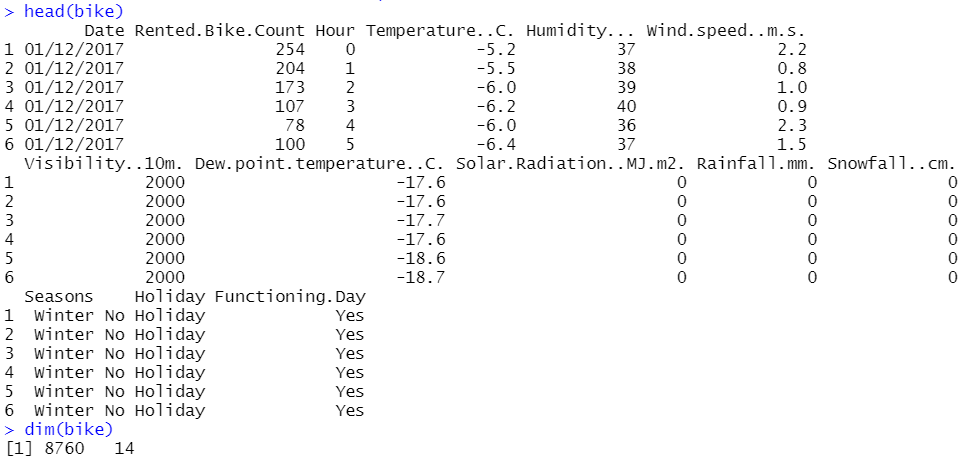
\includegraphics[width=0.7\linewidth]{../Photo Of Result/A2_head}
	\caption{Một vài quan trắc đầu tiên và số chiều của bộ dữ liệu ban đầu}
	\label{A2_head}
\end{figure}

Vì mục đích bài toán là dự đoán số lượng xe đạp theo mỗi giờ, do đó nhóm em loại bỏ biến \texttt{Date}. Bên cạnh đó, các biến định tính cũng được biến đổi thành các biến dummy để thuận tiện cho việc tính toán và hồi quy, cụ thể: biến \texttt{Hour} được phân rã thành 24 biến, biến \texttt{Seasons} được phân rã thành 4 biến, biến \texttt{Holiday} mang giá trị 1 nếu là Holiday và 0 nếu ngược lại, biến \texttt{Functional Day} mang giá~trị 1 nếu là Yes và 0 nếu ngược lại. Lúc này bộ dữ liệu gồm 39 biến.
\begin{figure}[H]
	\centering
	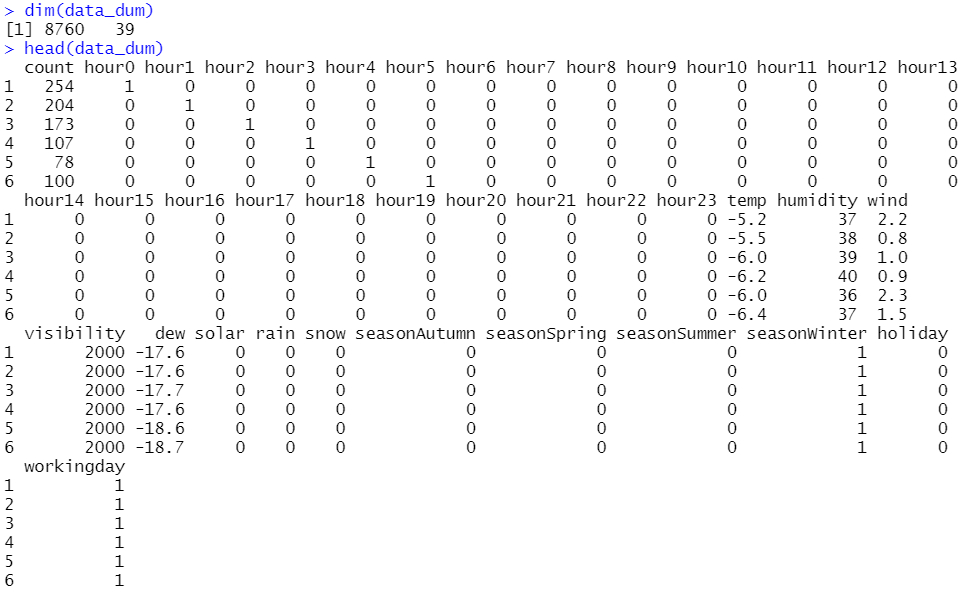
\includegraphics[width=0.7\linewidth]{../Photo Of Result/A2_dummy}
	\caption{Dữ liệu sau khi loại bỏ \texttt{Date} và tạo các biến giả}
	\label{A2_head2}
\end{figure}

\subsection*{Phân tích và chọn mô hình}

\begin{figure}[H]
	\centering
	{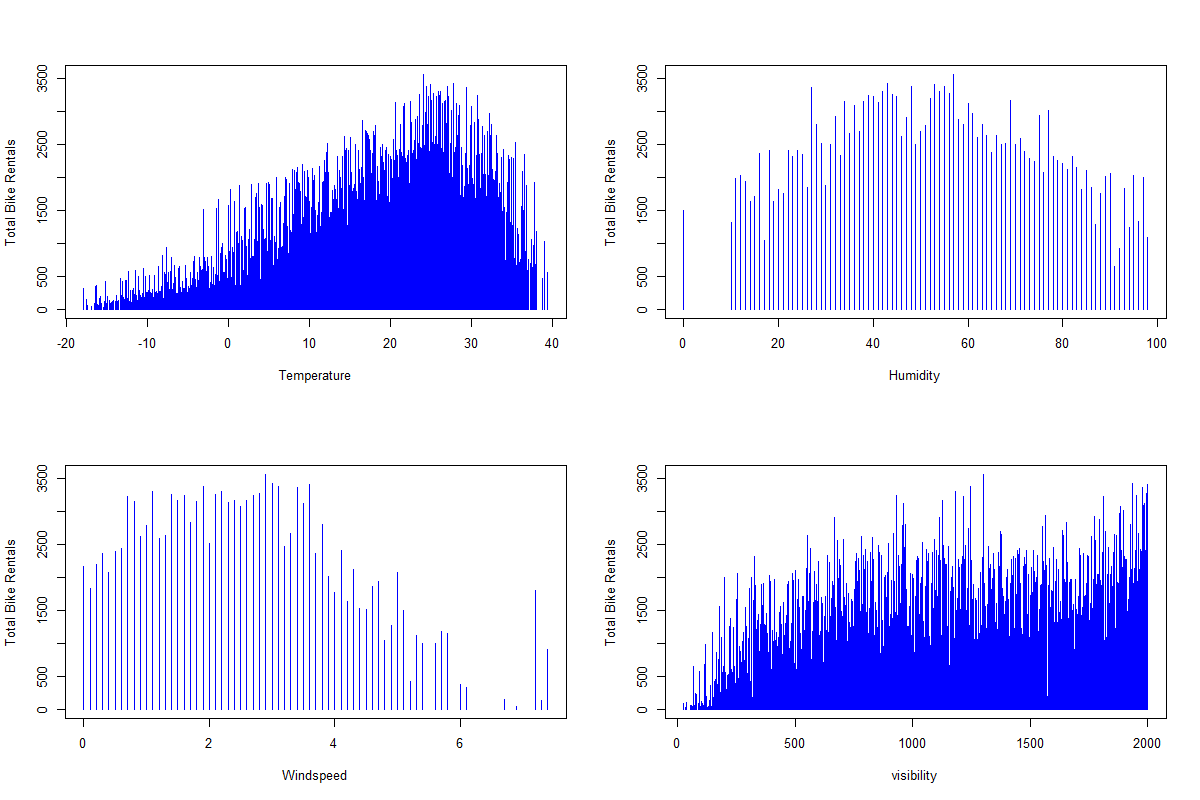
\includegraphics[width=.75\linewidth]{../Photo Of Result/A2_plotvar1}}\\
	{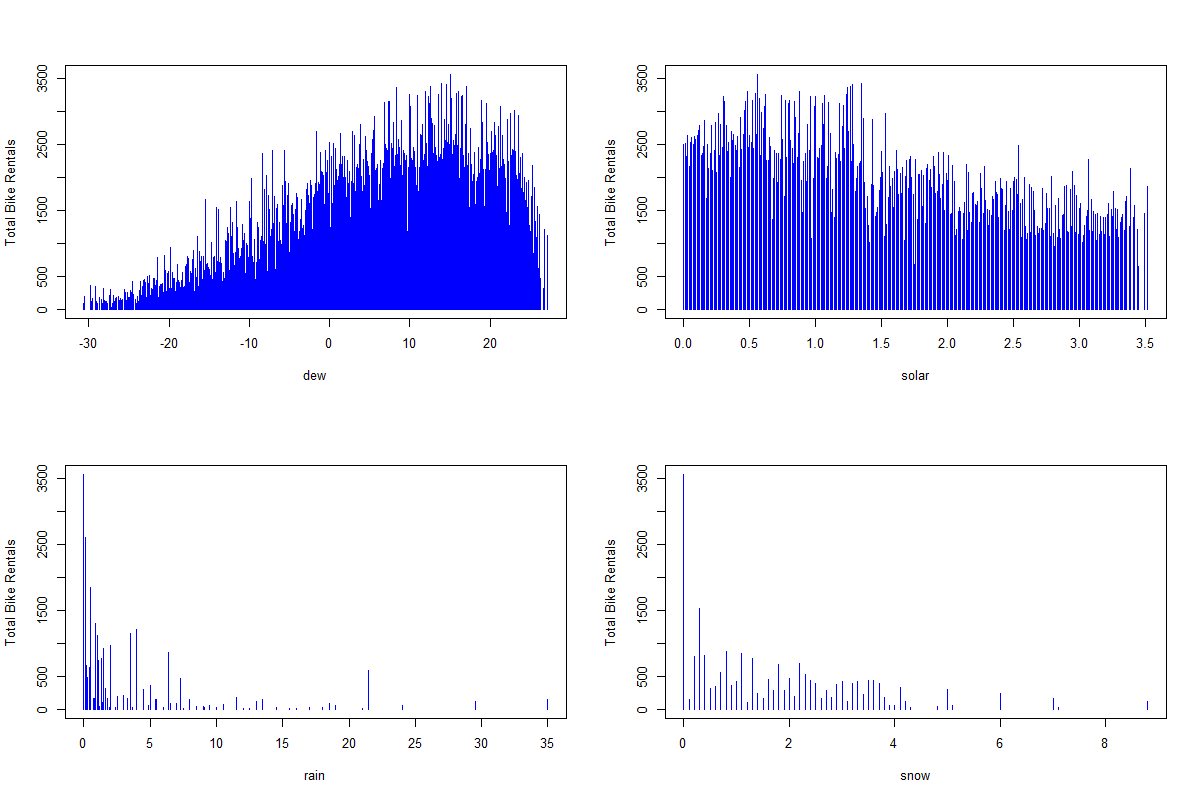
\includegraphics[width=.75\linewidth]{../Photo Of Result/A2_plotvar2}}
	\caption{Quan sát phân bố của từng biến với \texttt{Count}}
	\label{A2_visual1}
\end{figure}

Quan sát các kết quả ở hình \ref{A2_visual1} và \ref{A2_visual2}, có thể rút ra một số nhận xét như sau:
\begin{itemize}
	\item \texttt{Temp}, \texttt{Dew}: Nhiệt độ và nhiệt độ điểm sương có ảnh hưởng nhiều đến số lượng xe~đạp được thuê. Khi cả hai chỉ số nhiệt độ này quá thấp (dưới $0^oC$) hoặc quá cao thì số~lượng xe đạp được thuê khá ít, và số lượng xe đạp được thuê tăng dần khi các chỉ số nhiệt độ này nằm trong khoảng lý tưởng (từ $5^oC$ đến $25^oC$).
	\item \texttt{Humidity}, \texttt{Wind}, \texttt{Visibility}, \texttt{Solar}: Các yếu tố độ ẩm, tốc độ gió, tầm nhìn và bức xạ mặt trời có ảnh hưởng đến số lượng xe đạp được thuê nhưng không nhiều. Trong các trường hợp đặc biệt như tốc độ gió quá lớn hoặc tầm nhìn xa bị cản trở thì số lượng xe đạp được thuê bị giảm đi đáng kể. Điều này cũng khớp với thực tế, vì những điều kiện thời tiết này không thích hợp cho việc di chuyển bằng xe đạp.
	\item \texttt{Rain}, \texttt{Snow}: Lượng mưa và độ dày của tuyết có ảnh hưởng rõ rệt đến số lượng thuê xe đạp. Khi trời không mưa hoặc mưa ít, không có tuyết hoặc độ dày của tuyết không đáng kể, thì số lượng xe đạp được thuê khá cao. Và hiển nhiên, khi lượng mưa tăng, độ dày của tuyết tăng thì việc di chuyển bằng xe đạp dường như là rất~ít.
\end{itemize}

\begin{figure}[H]
	\centering
	{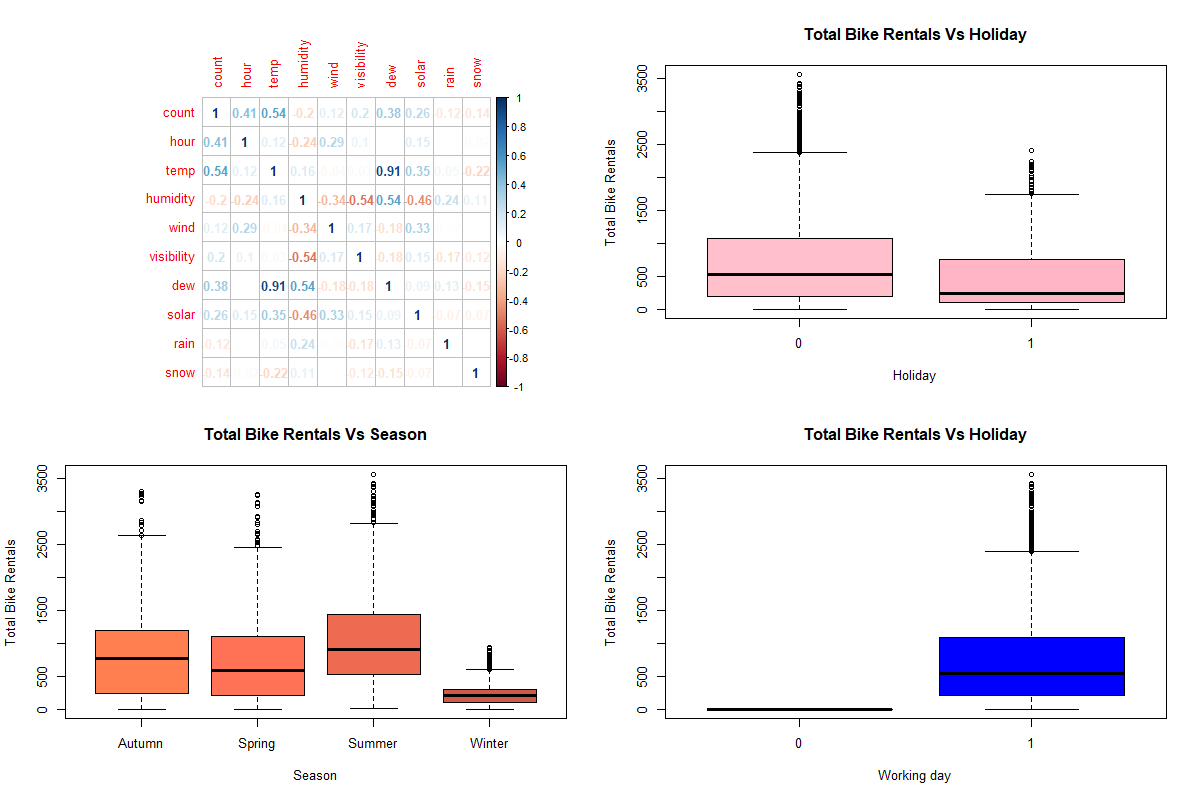
\includegraphics[width=\linewidth]{../Photo Of Result/A2_corr}}	
	\caption{Quan sát ma trận hệ số tương quan và các biến định tính}
	\label{A2_visual2}
\end{figure}

\begin{itemize}
	\item \texttt{Holiday}: Số lượng xe đạp được thuê trong các ngày lễ ít hơn so với ngày bình~thường.
	\item \texttt{Season}: Số lượng xe đạp được thuê trong bốn mùa là có sự chênh lệch, nhưng không nhiều. Xe đạp được thuê vào mùa đông (winter) ít hơn hẳn so với ba mùa còn lại, điều này cũng dễ hiểu và có thể giải thích thông qua các biến \texttt{Temp}, \texttt{Dew}, \texttt{Snow} như đã phân tích.
	\item \texttt{WorkingDay}: Vào những ngày không đi làm, số lượng xe đạp được thuê là cực ít.
\end{itemize}

Ma trận hệ số tương quan (hình \ref{A2_visual2}) cho thấy các yếu tố về giờ \texttt{Hour} và ghiệt độ \texttt{Temp} cũng có mối tương quan khá cao với số lượng xe đạp cho thuê \texttt{Count}; các biến nhiệt độ \texttt{Temp}, nhiệt độ điểm sương \texttt{Dew} và độ ẩm \texttt{Humidity} có mối tương quan cao với nhau, chứng tỏ có tồn tại hiện tượng đa cộng tuyến trong bộ dữ liệu. 

\begin{figure}[H]
	\centering
	\subfloat[Phân bố biến \texttt{Count} theo từng giờ]
	{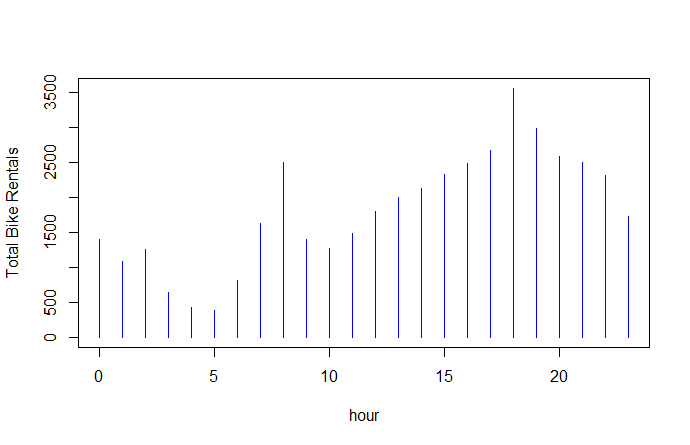
\includegraphics[width=.5\linewidth]{../Photo Of Result/A2_plot_hour}}	\hfill
	\subfloat[Phân bố biến \texttt{Count}]
	{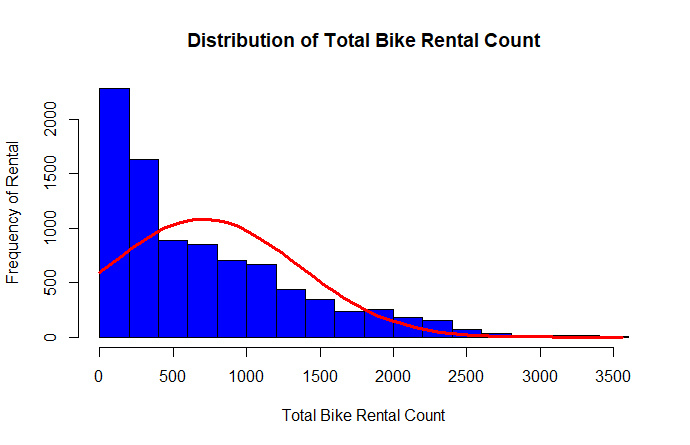
\includegraphics[width=.5\linewidth]{../Photo Of Result/A2_plotcount}}
	\caption{Quan sát phân bố biến phụ thuộc \texttt{Count}}
	\label{A2_visual3}
\end{figure}

Số lượng xe đạp cho thuê, \texttt{Count}, không tuân theo phân phối chuẩn, và bị lệch hẳn về một phía. Có thể thấy nhu cầu thuê xe đạp ở Seoul thông thường không quá 1000 chiếc vào mỗi giờ, và rất ít khi vượt quá 2500 chiếc (hình \ref{A2_visual3}). Ngoài ra, số lượng xe~đạp được thuê ở các giờ cũng có sự chênh lệch đáng kể. Xe được thuê nhiều vào khoảng $7-8$ giờ sáng, khi mọi người đi học đi làm; và vào khoảng $18-20$ giờ, khoảng thời gian tan học, tan làm.

\bigskip
Để giải quyết vấn đề của bộ dữ liệu có số lượng biến lớn và có mối tương quan mạnh giữa các biến độc lập với nhau, nhóm em dùng phương~pháp phân tích thành phần chính (PCA) để biến đổi dữ liệu về không gian có số chiều nhỏ hơn mà vẫn giữ được nhiều thông tin nhất có thể của bộ dữ liệu.

\begin{figure}[H]
	\centering
	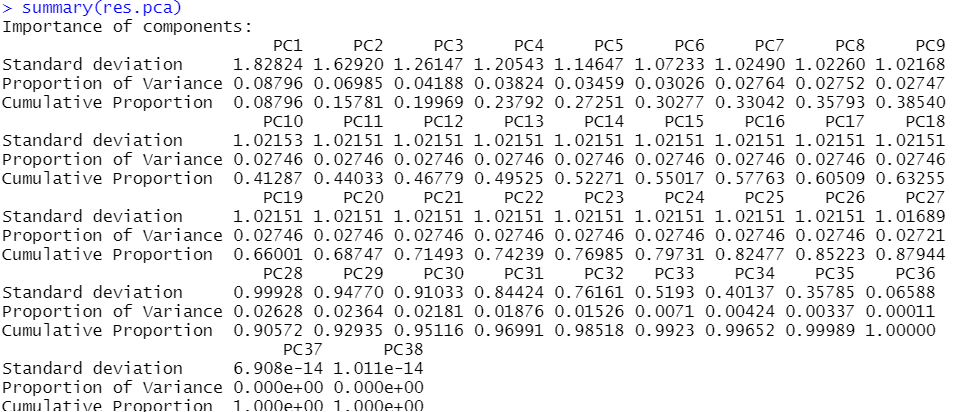
\includegraphics[width=0.8\linewidth]{../Photo Of Result/A2_PCproportion.PNG}
	\caption{Kết quả phân tích thành phần chính }
	\label{A2_Var}
\end{figure}

\begin{figure}[H]
	\centering
	\subfloat[Hồi quy với 26 thành phần chính đầu tiên]
	{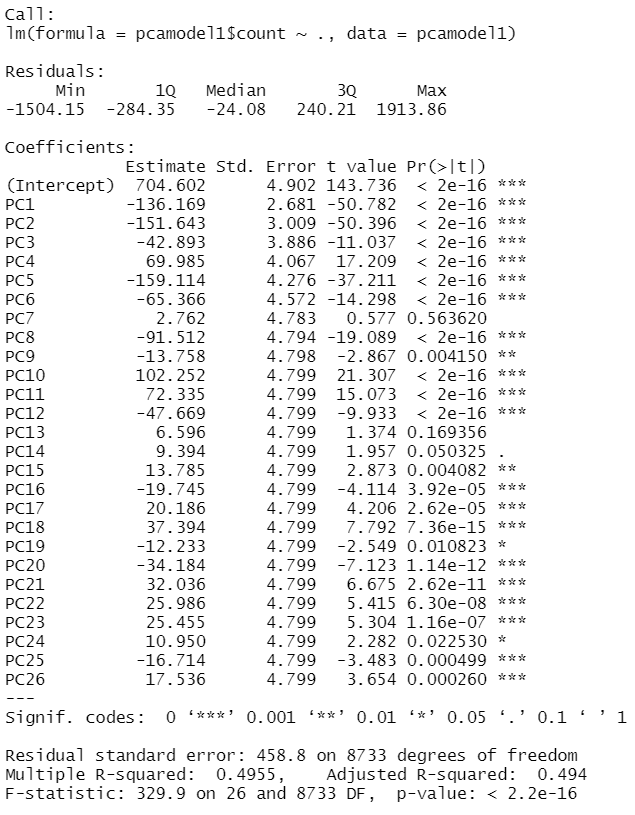
\includegraphics[width=0.5\linewidth]{../Photo Of Result/A2_pca_mod1.PNG}} \hfill
	\subfloat[Hồi quy với 23 thành phần chính]
	{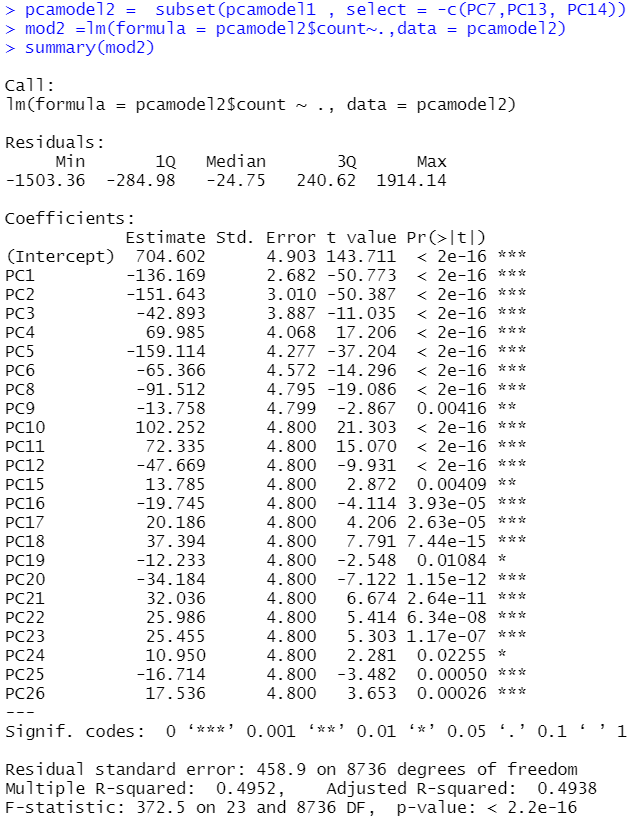
\includegraphics[width=0.5\linewidth]{../Photo Of Result/A2_pca_mod2.PNG}}
	\caption{Hồi quy thành phần chính}
	\label{A2_modPCA}
\end{figure}

Mô hình giải thích được khoảng $50\%$ cho sự thay đổi số lượng thuê xe đạp tại Seoul. Tuy nhiên, trong mô hình hồi quy có chứa các biến \texttt{PC7}, \texttt{PC13}, và \texttt{PC14} không có ý~nghĩa thống kê do $\rho_{value} \ge 5\%$. Tiến hành loại bỏ những biến này ra khỏi mô hình và thực hiện hồi quy tuyến tính trên tập các biến còn lại, ta thu được $R^{2} \approx 49.5\% $, không thay đổi nhiều so với mô~hình trước đó (hình \ref{A2_modPCA}.b), và trong mô hình mới này tất cả những biến độc lập đều có ý nghĩa thống kê do $\rho_{value} \ge 5\%$.

\begin{figure}[H]
	\centering
	{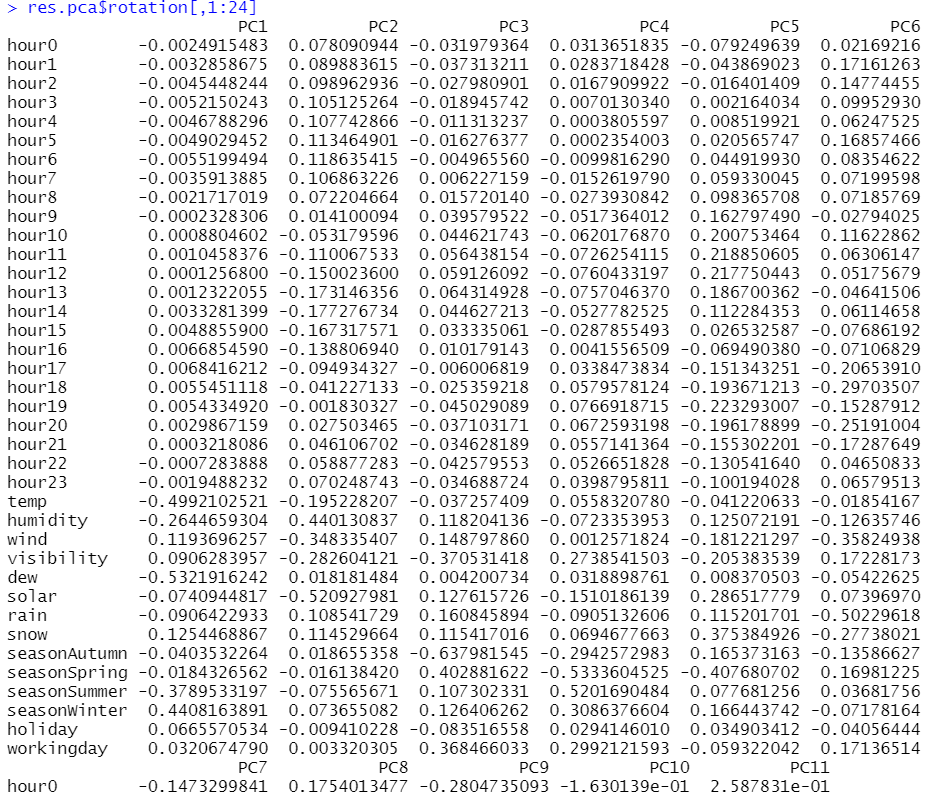
\includegraphics[width=.9\linewidth]{../Photo Of Result/A2_loading.PNG}}
	\caption{Phần trăm đóng góp của các biến trong các thành phần chính}
	\label{A2_loading}
\end{figure}

Dựa vào hình \ref{A2_loading} và \ref{A2_plot}. Các biến \texttt{Dew, Temp, SeasonSummer, SeasonWinter} đóng vai trò quan trọng trong việc giải thích thành phần chính thứ nhất, cụ thể:

$$\texttt{PC1} = -0.499 \times \texttt{Temp} -0.532 \times \texttt{Dew} -0.378 \times \texttt{SeasonSummer} + 0.440 \times \texttt{SeasonWinter}$$

Các biến \texttt{Solar, Humidity, Wind, Visibility} đóng vai trò quan trọng trong việc giải thích thành phần chính thứ hai, cụ thể:

$$\texttt{PC2} = 0.440 \times \texttt{Humidity} -0.348 \times \texttt{Wind} -0.520 \times \texttt{Solar} + 0.282 \times \texttt{Visibility}$$

\begin{figure}[H]
	\centering
	{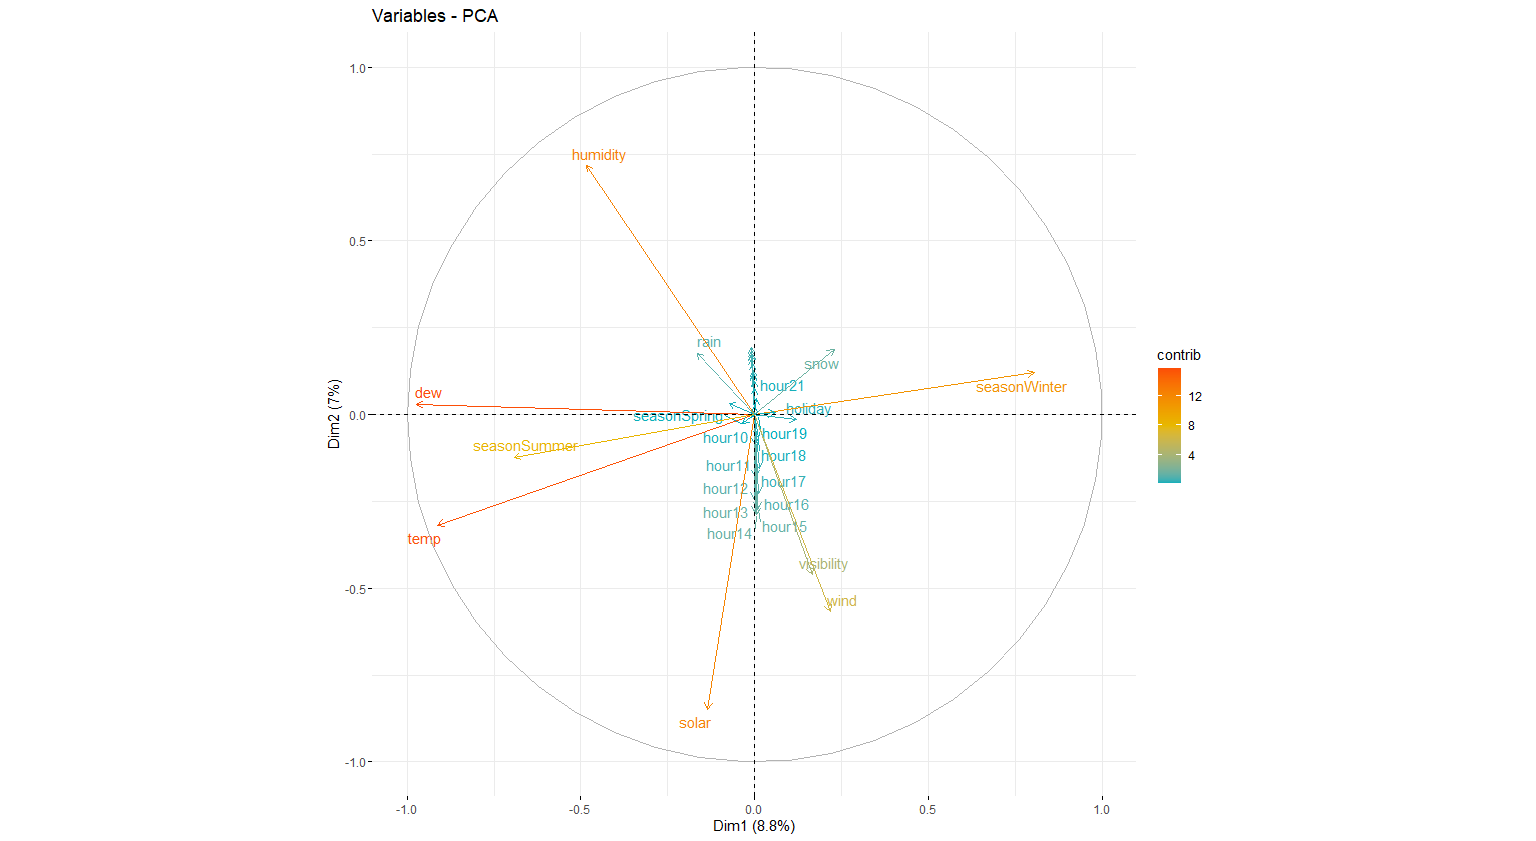
\includegraphics[width=.8\linewidth]{../Photo Of Result/A2_pca.PNG}}
	\caption{Biểu đồ biểu diễn hai thành phần chính đầu tiên}
	\label{A2_plot}
\end{figure}

\subsection*{Nhận xét và kết luận}

Thành phần chính thứ nhất có thể xem là yếu tố nhiệt độ, thành phần chính thứ hai có thể xem như yếu tố trạng thái thời tiết (xấu hay tốt, được giải thích bởi độ ẩm, gió, tầm nhìn và bức xạ mặt trời). Yếu tố thời gian, \texttt{Hour, WorkingDay, Holiday} cũng được biểu diễn thông qua thành phần chính thứ 2, nhưng độ đóng góp là không nhiều. 

Số lượng xe đạp cho thuê trong mỗi giờ chủ yếu bị ảnh hưởng bởi các yếu tố nhiệt~độ và trạng thái thời tiết, trong điều kiện thời tiết tốt thì số lượng thuê xe đạp sẽ tăng và ngược lại.
Mặc dù mô hình phân tích thành phần chính có thể giải thích khoảng 50\% sự biến thiên của số lượng xe đạp cho thuê, nhưng đây chưa phải là một kết quả cao, nhóm cũng chưa sử dụng mô hình cho việc dự đoán kiểm tra (testing). Tiến hành phân~tích thành phần chính đã làm triệt tiêu hiện tượng đa cộng tuyến trong mô hình. 

Tuy nhiên, sự tác động của biến \texttt{Hour} ở mô hình biến đổi không được thể hiện rõ như những phân tích ban đầu, vì biến này đã được chuyển thành những biến giả và độ đóng góp trong các thành phần chính là không đáng kể. Để phân tích và xây dựng mô~hình dự đoán tốt hơn, cần tiến hành phân tích thêm để loại bỏ các điểm bất thường, cũng như tìm cách xây dựng/biến đổi những biến ban đầu một cách hợp lý hơn.